\documentclass[10pt,twoside]{article}

\usepackage[margin=0.5in]{geometry}
\usepackage{epsfig}
\usepackage{calc}
\usepackage{amssymb}
\usepackage{amstext}
\usepackage{amsmath}
\usepackage{amsthm}
\usepackage{multicol}
\usepackage{pslatex}
\usepackage{apalike}
\usepackage{graphicx}
\usepackage{caption}
\usepackage{subcaption}
\begin{document}

\title{6.867 Machine Learning  \subtitle{Homework 2} }

\maketitle

% **************************************************************************************************
 % Problem 1
% **************************************************************************************************

\section{\uppercase{Logistic Regression}}

\noindent Logistic Regression is a discriminative model used for classification. Given an input x, it finds the posterior of x belonging to one of the classes and then uses that probability to classify x. In the simplest case, it takes the dot product of x and w and uses that as an input to the sigmoid function, which outputs a number between 0 and 1. An advantage of logistic regressions is that they have few parameters, which allows them to be trained relatively quickly. One of the problems with logistic regressions is that they are very prone to overfitting to the training data. One way to prevent the overfitting is to add a regularization term, lambda, which penalizes the size of the weight vector. The size of the weight vector can be penalized using the L1 norm of the L2 norm. Here, we explore how different lambda values and the different norms affect several aspects of the logistic regression.

\subsection{Optimizing with Gradient Descent}

\noindent To investigate how regularization affected the logistic regression we tried lambda values of 0 and 1. We decided not to penalize the bias term in the weight vector. As expected, we found that with a lambda value of 1 the weight vector decreased in every iteration of the algorithm. 


\subsection{Section1}

\subsection{Section2}


% **************************************************************************************************
 % Problem 2
% **************************************************************************************************

\section{\uppercase{Support Vector Machines}}

Support Vector Machines are supervised learning models that work by finding a dividing hyperplane between the training data while maximizing the gap between the training data and the decision boundary. This is to help the classifier generalize better and makes it more robust to noise. Assuming the data is linearly separable, finding this dividing hyperplane amounts to solving the quadratic program

% \begin{equation}
% \min_{w,b} \frac{1}{2} ||w||^2 s.t. y^i(w^T x^i + b) \gte 1, 1 \lte i \lte n
% \end{equation}

% \begin{equation}
% \begin{array}
% min \frac{1}{2} ||w||^2 &\\
% s.t. y^i(w^T x^i + b) \geq 1, 1 \leq i \leq n
% \end{array}
% \end{equation}

\begin{equation}
\begin{array}{ll@{}ll}
\text{min}  & \displaystyle \frac{1}{2} ||w||^2 &\\
\text{s. t.}& \displaystyle y^i(w^T x^i + b) \geq 1 , 1 \leq i \leq n
\end{array}
\end{equation}

where $w$ is the vector perpendicular to the dividing hyperplane and $\frac{1}{||w||}$ is the size of the margin.

If the data is almost but not completely linearly separable, we can still model the data with an SVM by introducing slack variables when solving for a classifier. We allow the training points to be misclassified by some amount $e$ and the goal is to maximize the margin while minimizing the slack. This formulation is called C-SVM and the separating hyperplane can be found by solving the quadratic program below.

\begin{equation}
\begin{array}{ll@{}ll}
\text{min}  & \displaystyle \frac{1}{2} ||w||^2 + C \sum_i e_i &\\
\text{s. t.}& \displaystyle y^i(w^T x^i + b) \geq 1 - e_i , 1 \leq i \leq n \\
& e_i \geq 0 , 1 \leq i \leq n
\end{array}
\end{equation}

\subsection{Dual Formulation of C-SVM}
This problem as stated above is difficult to implement with kernels functions. Fortunately, we convert the problem from the primal formulation stated above and instead implement its dual formuation.

\begin{equation}
\begin{array}{ll@{}ll}
\text{min}  & \displaystyle \frac{1}{2} \sum_{i=1}^{n} \sum_{j=1}^n \alpha_i \alpha_j y_i y_j [\phi(x_i)^T \phi(x_j)] - \sum_{t=1}^{n} \alpha_t &\\
\text{s. t.}& \displaystyle 0 \leq a_t \leq C , \sum_{t=1}^{n} \alpha_t y_t = 0
\end{array}
\end{equation}

To solve this linear program and get the $\alpha$s, we used the solver in a python library called cvxopt. The solver finds solutions to quadratic programs of the form:

\begin{equation}
\begin{array}{ll@{}ll}
\text{min}  & \displaystyle \frac{1}{2} x^T P x + q^T x &\\
\text{s. t.}& \displaystyle G x \leq h &\\
& Ax = b
\end{array}
\end{equation}

In our case, our matrices are 

\begin{equation*}
P = Diag(\overrightarrow{y}) X X^T Diag(\overrightarrow{y})
\end{equation*}
\begin{equation*}
q = -1 * \overrightarrow{1}
\end{equation*}
\begin{equation*}
G = [I | -I]
\end{equation*}
\begin{equation*}
h = [C * \overrightarrow{1} | \overrightarrow{0}]
\end{equation*}
\begin{equation*}
A = \overrightarrow{y}
\end{equation*}
\begin{equation*}
b = 0
\end{equation*}

$Diag(\overrightarrow{y})$ is a diagonal matrix with $y^{(i)}$s on the diagonal.

This solver returns $\overrightarrow{x}$ which is our $\overrightarrow{\alpha}$ vector. Testing this implementation,

Do the stupid example!

\subsection{2D Dataset Results}
\begin{figure}
        \begin{subfigure}[b]{0.25\textwidth}
                \centering
                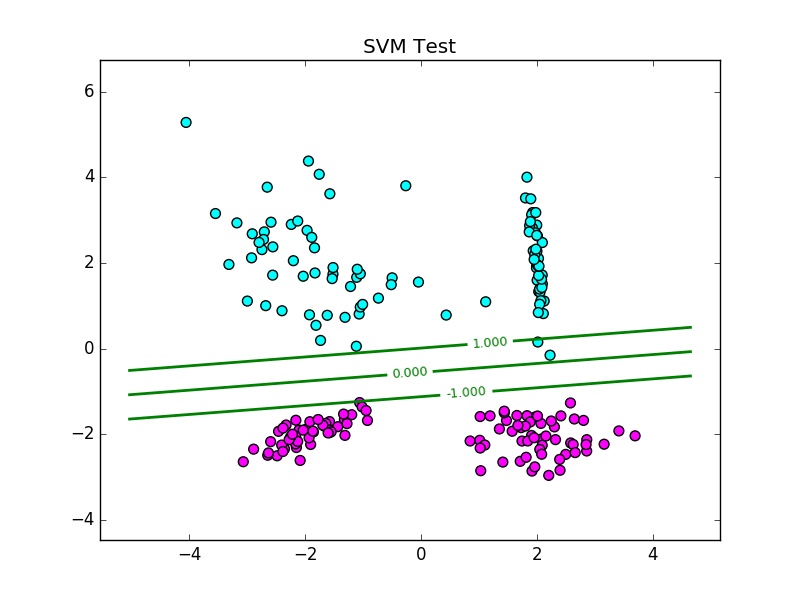
\includegraphics[width=\linewidth]{Figures/P2/svm_data1_test_C1.png}
                \caption{A gull}
                \label{fig:gull}
        \end{subfigure}%
        \begin{subfigure}[b]{0.25\textwidth}
                \centering
                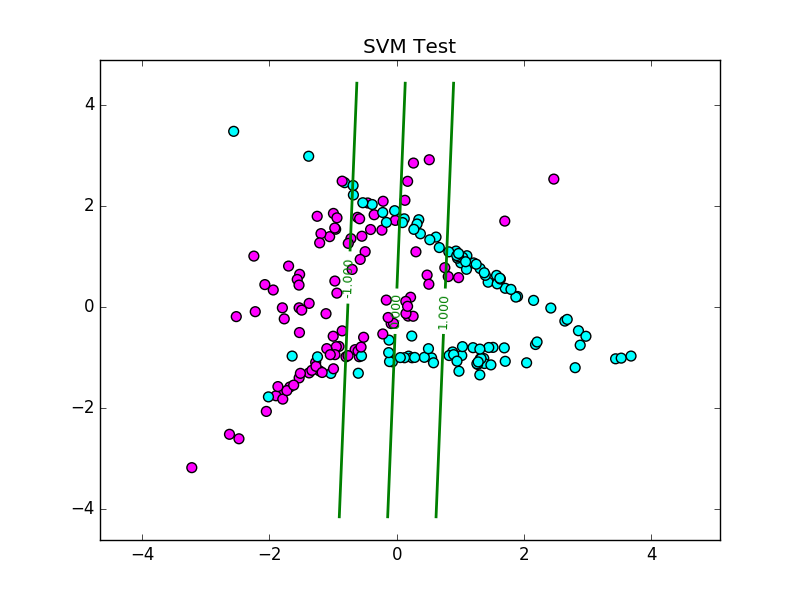
\includegraphics[width=\linewidth]{Figures/P2/svm_data2_test_C1.png}
                \caption{A gull2}
                \label{fig:gull2}
        \end{subfigure}%
        \begin{subfigure}[b]{0.25\textwidth}
                \centering
                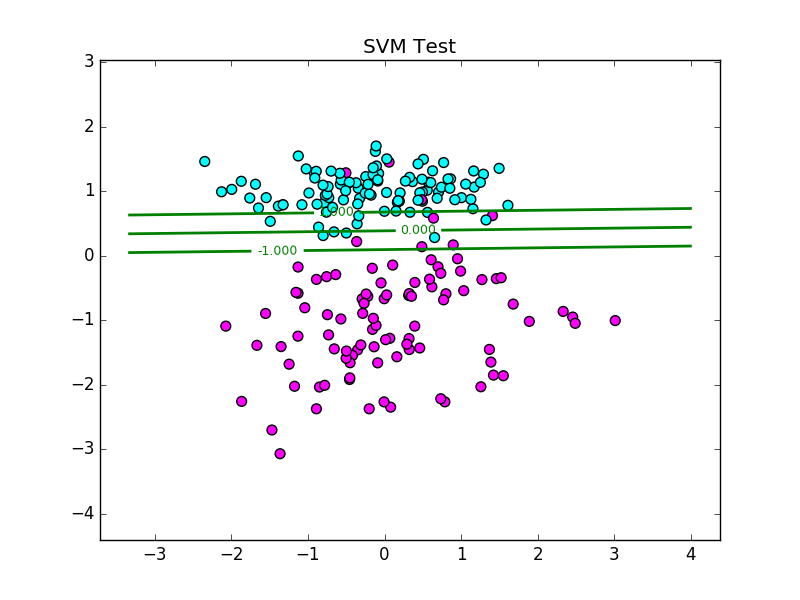
\includegraphics[width=\linewidth]{Figures/P2/svm_data3_test_C1.png}
                \caption{A tiger}
                \label{fig:tiger}
        \end{subfigure}%
        \begin{subfigure}[b]{0.25\textwidth}
                \centering
                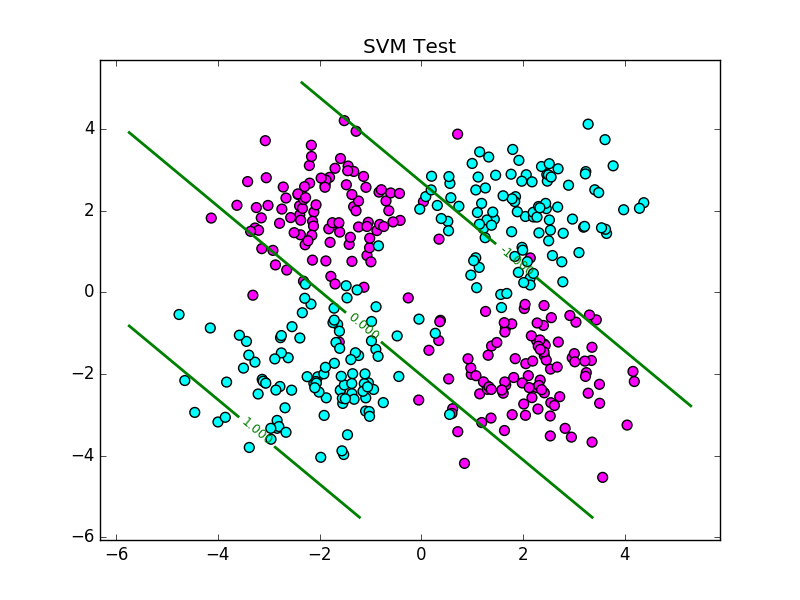
\includegraphics[width=\linewidth]{Figures/P2/svm_data4_test_C1.png}
                \caption{A mouse}
                \label{fig:mouse}
        \end{subfigure}
        \caption{Pictures of animals}\label{fig:animals}
\end{figure}

\subsection{2D Dataset Results with Kernel Functions}



% **************************************************************************************************
 % Problem 3
% **************************************************************************************************

\section{\uppercase{Support Vector Machine with Pegasos}}

\subsection{Section1?}


\subsection{Section2?}


% **************************************************************************************************
 % Problem 4
% **************************************************************************************************

\section{\uppercase{Handwritten Digit Recognition with MNIST}}


\vfill
\end{document}

